\documentclass[11pt, a4paper, french]{thesul}
\newcommand{\TitreThese}{
Manipulation et refroidissement par �vaporation forc�e d'ensembles atomiques ultra-froids pour la production d'un jet intense dans le r�gime de d�g�n�rescence quantique : vers l'obtention d'un \textit{laser � atomes continu}}

\usepackage{ifthen}
\usepackage{ifpdf}

%\usepackage[pdftex]{thumbpdf}
\usepackage[pdftex]{graphicx} % pour l'incusion de graphiques


\graphicspath{{images/}}
%\setkeys{Gin}{width=\linewidth}

\usepackage[intlimits]{amsmath}
\usepackage{amssymb}
% pour des repr�sentation de vecteur sympa pour les physiciens
\usepackage{vector}
\usepackage{array}
\usepackage{slashbox}% pour couper une case de tableau en deux

% figures avec sous-figures et sous-captions:
\usepackage[subrefformat=subparens]{subfig}

% pour des r�f�rences en language naturel
\usepackage[english]{varioref} 

% pour des supers graphiques trop cool, mieux que PSTricks
\usepackage{tikz,tkz-fct,tkz-2d}
\usetikzlibrary{shapes,snakes,arrows,patterns}

\usepackage[np,autolanguage]{numprint}

\usepackage[autoplay, loop, poster]{animate} % pour animer des dessins

% texte sur des images
\usepackage[abs]{overpic}
\setlength\unitlength{1cm}

%%%%%%%%%%%%%%%%%%%%%%%%%%%%%%%%%%%%%%%%%%%%%%%%%%%%%%%
% Pour pouvoir avoir des fleche depuis le texte vers des formule par exemple:
% http://www.fauskes.net/pgftikzexamples/global-nodes/
%%%%%%%%%%%%%%%%%%%%%%%%%%%%%%%%%%%%%%%%%%%%%%%%%%%%%%%
% For every picture that defines or uses external nodes, you'll have to apply the 'remember picture' style. To avoid some typing, we'll apply the style to all pictures.
\tikzstyle{every picture}+=[remember picture] 
% By default all math in TikZ nodes are set in inline mode. Change this to displaystyle so that we don't get small fractions.
\everymath{\displaystyle}

% espace int�ligent pour la fin d'une nexcommand en text
\usepackage{xspace}

%gestion des unit� !
\usepackage[amssymb]{SIunits}
\usepackage{sistyle}
\SIstyle{German} 

\usepackage{picins}
\usepackage{fancybox}

\usepackage{movie15}
% hachurer du texte avec \sout{Texte � barrer}\xout{Texte � hachurer}\uwave{Texte � souligner par une vaguelette}
\usepackage[normalem]{ulem}


% pour ajouter localement une ligne � une page
% contient une commande pour checker si on est sur un page odd or even
\usepackage{addlines}
\usepackage{mparhack}

% Si on veut des mini-tables des matieres (utiliser minitoc-hyper en conjonction avec tlhypref) :
\ifpdf % le monde PDF
\usepackage[english]{minitoc-hyper}
\else % le monde DVI/PS
\usepackage[english]{minitoc}
\fi

% Liste notations
\usepackage[refpage,english,intoc]{nomencl}  %intoc rajoute une ligne dans la toc

%\usepackage{tocbibind}                     % toc,lotf,bib,index in toc
%\usepackage[numbers,sort&compress]{natbib} % Good [47] type referencing
%\usepackage{hypernat}                      % Makes natbibs s&c play w/ hyperref

\ifpdf % le monde PDF
%\usepackage{hyperref} % pour des r�f�rences cliquables
\usepackage[pdftex, colorlinks = true
%						, pdfstartview = FitH
%						, colorlinks=false,
						, linkcolor = blue, citecolor = blue, urlcolor = blue, pdfpagelabels, pagebackref]{tlhypref}
\hypersetup{pdfauthor={Gael Reinaudi},
pdftitle={\TitreThese},
pdfsubject={Th�se de doctorat},
pdfkeywords={physique,quantique,laser,atome,d�g�n�rescence,froid,manipulation,atomique,refroidissement,�vaporation,jet}}
\else % le monde DVI/PS
\fi
% ********************************************************************
% get the links to the figures and tables right
%\RequirePackage[all]{hypcap} % to be loaded after hyperref package
% ********************************************************************
% setup the style of the backrefs from the bibliography
\newcommand{\backrefnotcitedstring}{\relax}%(Not cited.)
\newcommand{\backrefcitedsinglestring}[1]{Cit� � la page~#1.}
\newcommand{\backrefcitedmultistring}[1]{Cit� aux pages~#1.}
\RequirePackage[hyperpageref]{backref} % to be loaded after hyperref package
   \renewcommand{\backreftwosep}{ et~} % seperate 2 pages
   \renewcommand{\backreflastsep}{, et~} % seperate last of longer list
   \renewcommand*{\backref}[1]{}  % Disable standard
   \renewcommand*{\backrefalt}[4]{% Detailed backref
      \ifcase #1 %
         \backrefnotcitedstring%
      \or
         \backrefcitedsinglestring{#2}%
      \else
         \backrefcitedmultistring{#2}%
      \fi} 
% ********************************************************************

% Si l'on produit le PDF avec pdflatex, ceci remplace la plupart
% des polices EC par des polices CM, plus adaptees a la generation de PDF,
% car ayant des equivalents PS :
\usepackage{aeguill}
% Pour tout savoir sur les polices
% (cette ligne n'est pas necessaire au traitement du fichier)
%\usepackage[infoshow]{tracefnt}

% �vite les under-over full box...
%\usepackage[auto=false]{microtype} % 2010-05-27
%\usepackage{microtype}

\usepackage[T1]{fontenc}
\usepackage[latin1]{inputenc}
\usepackage{lmodern}



%%% Pour n'avoir que l'image tikz ! ! !
\usepackage[active,tightpage]{preview}\PreviewEnvironment{tikzpicture} 

\usepackage[np,autolanguage]{numprint}
\begin{document}
\pagestyle{empty}
\newcommand\FaitNomenclature{1}
\newcommand\FaitNomEnMarge{1}

\renewcommand{\emph}[1]{\textbf{\textit{{#1}}}}
\providecommand{\enquote}[1]{``#1''}

\newcommand{\termetech}[1]{\textit{{#1}}}
\newcommand{\nomofficiel}[1]{\textit{{#1}}}
\newcommand{\sotosay}[1]{\enquote{\textit{{#1}}}}
\newcommand{\parole}[1]{\og\textit{{#1}}\fg}

\newenvironment{itemizel}%
   {\begin{itemize}}{\end{itemize}\vspace*{1.5ex}}%

\newenvironment{ditemize}%
%   {\begin{list}%
%   {$\bullet$}{}%
%   }{\end{list}}%
   {\begin{itemize}}{\end{itemize}}%

% ************************************************************************
\newcommand{\casse}{\pagebreak}
% ************************************************************************
\newcommand{\bfig}{\begin{GaelFigure}}
\newcommand{\bfigs}{\bfig\RemonteUnPeuFig}
\newcommand{\bfigss}{\bfigs\RemonteUnPeuFig}
\newcommand{\bfigsss}{\bfigss\RemonteUnPeuFig}
\newcommand{\bfighs}{\bfigh\RemonteUnPeuFig}
\newcommand{\bfighss}{\bfighs\RemonteUnPeuFig}
\newcommand{\bfighsss}{\bfighss\RemonteUnPeuFig}
\newcommand{\CaptionFigs}[1]{\RemonteUnPeuFig \CaptionFig{#1}}
\newcommand{\CaptionFigss}[1]{\RemonteUnPeuFig \CaptionFigs{#1}}
\newcommand{\CaptionFigsss}[1]{\RemonteUnPeuFig \CaptionFigss{#1}}
\newcommand{\CaptionFigssss}[1]{\RemonteUnPeuFig \CaptionFigsss{#1}}

\newcommand{\efig}{\end{GaelFigure}}
\newcommand{\bfigh}{\begin{GaelFigureh}}
\newcommand{\efigh}{\end{GaelFigureh}}

\newcommand{\inlinefigr}[1]{\parpic[r,s]{{#1}}}
\newcommand{\inlinefigl}[1]{\parpic[l,s]{{#1}}}
\newcommand{\inlinefig}[1]{\inlinefigr{#1}}

% Pour enlever toutes les figures !
%\renewcommand{\includegraphics}[2][]{}\renewcommand{\animategraphics}[5][]{}
   
% Des notes pour donner des points de repere dans les cahier de labo.
% A commenter pour la version publique
\newcommand{\Cahier}[1]{%
%{\color{red}{CAHIER,PAGE #1}}%
}
% Des notes pour Gael.
% A commenter pour la version publique
\newcommand{\NoteGael}[1]{%
%{\color{magenta}{NOTE GAEL : \noindent #1 }}%
}
% Supprime de la version compil�e ce qu'il y a en argument
\newcommand{\EnFaitNon}[1]{}

% Les copi�s coll�s de TTL au cas o�
\newcommand{\dixit}[1]{#1}

% Les r�f�rences sans page
\newcommand{\nref}[1]{\ref{#1}}

\newcommand{\ttfrac}[2]{{{#1} / {#2}}}
%\newcommand{\ttfrac}[2]{{\sfrac{#1}{#2}}}

\newcommand{\AnimateOnline}{{(Animation en ligne) }}

%%%%%%%%%%%%%%%%%%%%%%%%%%%%%%%%%%%%%%%%%%%%%%%%%%%%%%%
% TIKZ : Pour pouvoir avoir des supers jolies boites avec du texte et des formule exemple:
% http://www.fauskes.net/pgftikzexamples/boxes-with-text-and-math/
%%%%%%%%%%%%%%%%%%%%%%%%%%%%%%%%%%%%%%%%%%%%%%%%%%%%%%%
\newcommand{\nResultat}[1]{#1}
\newcommand{\nRemarque}[1]{#1}
\newcommand{\nRemarqueTitre}[2]{\subsubsection{#1}#2}
\newcommand{\nnRemarque}[1]{}
\newcommand{\nnRemarqueTitre}[2]{}
%%%%%%%%%%%%%%%%%%%%%%%%%%%%%%%%%%%%%%%%%%%%%%%%%%%%%%%
% Boite d'Intuition
% Define box and box title style
\tikzstyle{IntuitionBox}=[draw=black, fill=green!05, very thick, 
rectangle, rounded corners, inner sep=10pt, inner ysep=13pt]
\tikzstyle{IntuitionTitre}=[draw=black, very thick, fill=white, text=black]
%\newcommand{\Intuition}[1]{%
%\begin{center}\begin{tikzpicture}
%\node [IntuitionBox] (box){%
%	\begin{minipage}{0.85\textwidth}%
%		{\color{black}{#1}%
%		\newpage}%
%		\vspace{-5pt}%
%	\end{minipage}};%
%\node[IntuitionTitre, anchor=center] at (box.north)
%{De mani�re qualitative...};
%\end{tikzpicture}\end{center}
%}

%%%%%%%%%%%%%%%%%%%%%%%%%%%%%%%%%%%%%%%%%%%%%%%%%%%%%%%
% Boite de Resultat important
\tikzstyle{ResultatBox}=[draw=red, fill=red!5, very thick,
    rectangle, rounded corners, inner sep=10pt, inner ysep=10pt]
\tikzstyle{ResultatTitre}=[fill=red, text=black]
\newcommand{\Resultat}[1]{%
\begin{center}\begin{tikzpicture}%
\node [ResultatBox] (box){%
	\begin{minipage}{0.85\textwidth}%
		{\color{black}{#1}%
		\newpage}%
	\end{minipage}};%
%\node[ResultatTitre, right=10pt] at (box.north west) {R�sultat};
\end{tikzpicture}\end{center}
}

%%%%%%%%%%%%%%%%%%%%%%%%%%%%%%%%%%%%%%%%%%%%%%%%%%%%%%%
% Boite d'Application num�rique
\tikzstyle{ApplicationNumeriqueBox}=[draw=black!20!green, fill=green!2, thick,
    rectangle, inner sep=10pt, inner ysep=13pt]
\tikzstyle{ApplicationNumeriqueTitre}=[draw=black!20!green, thick
, fill=white, text=black]
\newcommand{\ApplicationNumerique}[1]{%
\begin{center}\begin{tikzpicture}
\node [ApplicationNumeriqueBox] (box){%
	\begin{minipage}{0.85\textwidth}%
		{\color{black}{#1}%
		\newpage}%
		\vspace{-5pt}%
	\end{minipage}};%
\node[ApplicationNumeriqueTitre, right=10pt] at (box.north west)%
{Application num�rique};
\end{tikzpicture}\end{center}
}
\newcommand{\ApplicationNumeriqueTitre}[2]{%
\begin{center}\begin{tikzpicture}
\node [ApplicationNumeriqueBox] (box){%
	\begin{minipage}{0.85\textwidth}%
		{\color{black}{#2}%
		\newpage}%
		\vspace{-5pt}%
	\end{minipage}};%
\node[ApplicationNumeriqueTitre, right=10pt] at (box.north west)%
{Application num�rique : #1};
\end{tikzpicture}\end{center}
}

%%%%%%%%%%%%%%%%%%%%%%%%%%%%%%%%%%%%%%%%%%%%%%%%%%%%%%%
% Boite de Remarque
\tikzstyle{RemarqueBox}=[fill=blue!5, 
rectangle, inner sep=5pt, inner ysep=5pt]
\tikzstyle{RemarqueTitre}=[draw=white, thick, fill=white, text=black]
\tikzstyle{RemarqueLigne}=[color=blue
]%, very thick, cap=round]
\newcommand{\Remarque}[1]{%
\begin{center}\begin{tikzpicture}
\node [RemarqueBox, below right] (box)
{%
	\begin{minipage}{0.85\textwidth}%
		{\color{black}{#1}%
		\newpage}%
	\end{minipage}%
};
\node[RemarqueTitre, above right] at (box.north west) {Remarque};
\draw[RemarqueLigne] (box.north west)++(0,0.6)--(box.south west);
\draw[RemarqueLigne] (box.north west)--++(2,0);
\draw (box.south west)++(-1.5pt,0)--(-1.5pt,0.6);
%\draw[very thick] (box.north east)--(box.south east);
\end{tikzpicture}\end{center}
}
\newcommand{\RemarqueTitre}[2]{%
\begin{center}\begin{tikzpicture}
\node [RemarqueBox, below right] (box)
{%
	\begin{minipage}{0.85\textwidth}%
		{\color{black}{#2}%
		\newpage}%
	\end{minipage}%
};
\node[RemarqueTitre, above right] at (box.north west) {Remarque : {\textbf{#1}}};
\draw[RemarqueLigne] (box.north west)++(0,0.6)--(box.south west);
\draw[RemarqueLigne] (box.north west)--++(2,0);
\draw (box.south west)++(-1.5pt,0)--(-1.5pt,0.6);
\end{tikzpicture}\end{center}%
}
%%%%%%%%%%%%%%%%%%%%%%%%%%%%%%%%%%%%%%%%%%%%%%%%%%%%%%%%%%%%%%%%%%%%%%%%%%%%
%%%%%%%%%%%%%%%%%%%%%%%%%%%%%%%%%%%%%%%%%%%%%%%%%%%%%%%%%%%%%%%%%%%%%%%%%%%%
%%%%%%%%%%%%%%%%%%%%%%%%%%%%%%%%%%%%%%%%%%%%%%%%%%%%%%%%%%%%%%%%%%%%%%%%%%%%
%%%%%%%%%%%%%%%%%%%%%%%%%%%%%%%%%%%%%%%%%%%%%%%%%%%%%%%%%%%%%%%%%%%%%%%%%%%%
%%%%%%%%%%%%%%%%%%%%%%%%%%%%%%%%%%%%%%%%%%%%%%%%%%%%%%%%%%%%%%%%%%%%%%%%%%%%
\newcommand{\finformule}{\vspace{-3ex}}
\newcommand{\ff}{\finformule}
\newcommand{\RemonteUnPeuFig}{\vspace{-.2cm}}
\newcommand{\RemonteUneLigne}{\vspace{-3ex}}
\newcommand{\AjouteLigne}{\enlargethispage{1\baselineskip}}
\newcommand{\RetireLigne}{\enlargethispage{-1\baselineskip}}

\newenvironment{fminipage}{%
\begin{Sbox}\begin{minipage}}
{%
\end{minipage}\end{Sbox}
\shadowbox{\TheSbox}}

% Les figures � gael******************************************************
\newcommand{\MinipageWidth}{15cm}
\newcommand{\CaptionWidth}{14.6cm}
\newcommand{\CaptionMargin}{0.2cm}
\newcommand{\FigWidth}{14.5cm}
\newcommand{\FigWidthSansCm}{14.5}
\newcommand{\CaptionFig}[1]{\caption{\small{#1}}}
\newcommand{\CaptionTocCaptionFig}[2]{\caption[#1]{\small{#2}}}
\newcommand{\SansCaption}{\vspace{-0.24cm}}
% Les figures � gael******************************************************
\newenvironment{GaelFigure}[1][\MinipageWidth]{%
\begin{figure}[htbp]
\centering
\begin{fminipage}{#1}
\centering
\vspace{\CaptionMargin}
\pgfmathqparse{#1-\CaptionMargin-\CaptionMargin}
\begin{minipage}{\pgfmathresult pt}
\centering
}{%
\end{minipage}
\end{fminipage}
\end{figure}}
% Les figures � gael******************************************************
\newenvironment{GaelFigureh}[1][\MinipageWidth]{%
\begin{figure}[!ht]
\centering
\begin{fminipage}{#1}
\centering
\vspace{\CaptionMargin}
\pgfmathqparse{#1-\CaptionMargin-\CaptionMargin}
\begin{minipage}{\pgfmathresult pt}
\centering
}{%
\end{minipage}
\end{fminipage}
\end{figure}}

% ************************************************************************

%%%%%%%%%%%%%%%%%%%%%%%%%%%%%%%%%%%%%%%%%%%%%%%%%%%%
%% Pour faire des supers fleche d'hilight entre texte et �quation %%
%% http://www.fauskes.net/pgftikzexamples/global-nodes/
%% On d�finit un bout de fleche, et un d�part de fleche, puis on dit de faire les fleches....

\newcommand{\DepartHighlightColor}[2]%
{\tikz[baseline=(From#1.base)] {\node[fill=#1!10](From#1){#2};}}
%{#2}
\newcommand{\ArriveeHiglightColor}[2]%
{\tikz[baseline=(To#1.base)] {\node[fill=#1!10](To#1){#2};}}
%{#2}

\newcommand{\DepartHighlightColorMath}[2]{\DepartHighlightColor{#1}{\ensuremath{#2}}}%
\newcommand{\ArriveeHiglightColorMath}[2]{\ArriveeHiglightColor{#1}{\ensuremath{#2}}}%

\newcommand{\MakeFlecheHighlightColor}[1]%
{ \begin{tikzpicture}
[overlay]\path[->,opacity=0.5](From#1)edge%[bend left]
(To#1);
\end{tikzpicture}}
%{}

%%%%%%%%%%%%%%%%%%%%%%%%%%%%%%%%%%%%%%%%%%%%%%%%%%%%%%%%%%%%%%
%%%%%%%%% New commande pour le  texte%%%%%%%%%%%%%%%%%%%%%%%%%%%
\newcommand{\dgo}{David Gu�ry-Odelin\xspace}
\newcommand{\exatf}{exp�rience d'atome froids\xspace}
\newcommand{\exatfs}{exp�riences d'atome froids\xspace}
\newcommand{\thiq}{thermique\xspace}
\newcommand{\thdy}{thermodynamique\xspace}
\newcommand{\eqthdy}{�quilibre \thdy}
\newcommand{\reflab}{r�f�rentiel du laboratoire\xspace}
\newcommand{\refmir}{r�f�rentiel du miroir\xspace}
\newcommand{\dB}{de Broglie\xspace}

\newcommand{\tf}{transform�e de Fourier\xspace}

\newcommand{\rf}{radio-fr�quence\xspace}
\newcommand{\rfs}{{\rf}{s}\xspace}
\newcommand{\crf}{couteau \rf}
\newcommand{\hf}{hyperfin\xspace}
\newcommand{\hfs}{{\hf}{s}\xspace}
\newcommand{\sn}{sous-niveau\xspace}
\newcommand{\snx}{\sn{x}\xspace}
\newcommand{\snZ}{\sn Zeeman\xspace}
\newcommand{\snZs}{\snx Zeeman\xspace}
\newcommand{\snhf}{{\sn} \hf}
\newcommand{\snhfs}{{\snx} \hfs}

\newcommand{\ZS}{ralentisseur � effet Zeeman\xspace}

\newcommand{\rb}{rubidium\xspace}
\newcommand{\Rb}{$^{87}$Rb\xspace}
\newcommand{\RbCinq}{$^{85}$Rb\xspace}
\newcommand{\bec}{condensat de Bose-Einstein\xspace}
\newcommand{\becc}{condensat\xspace}
\newcommand{\beccs}{{\becc}s\xspace}
\newcommand{\becs}{condensats de Bose-Einstein\xspace}
\newcommand{\cbe}{condensation de Bose-Einstein\xspace}
\newcommand{\condbe}{\cbe}
\newcommand{\lat}{{laser � atomes}\xspace}
\newcommand{\lats}{{lasers � atomes}\xspace}
\newcommand{\rdq}{r�gime de d�g�n�rescence quantique\xspace}

\newcommand{\seqexp}{s�quence exp�rimentale\xspace}
\newcommand{\seqexps}{s�quences exp�rimentales\xspace}
\newcommand{\cdm}{centre de masse\xspace}

\newcommand{\ud}{unidimensionnel\xspace}
\newcommand{\ude}{unidimensionnelle\xspace}
\newcommand{\uds}{unidimensionnels\xspace}
\newcommand{\bd}{bidimensionnel\xspace}
\newcommand{\bde}{bidimensionnelle\xspace}
\newcommand{\bds}{bidimensionnels\xspace}
\newcommand{\td}{tridimensionnel\xspace}
\newcommand{\tde}{tridimensionnelle\xspace}
\newcommand{\tds}{tridimensionnels\xspace}

\newcommand{\reth}{rethermalisation\xspace}
\newcommand{\rether}{rethermaliser\xspace}
\newcommand{\cad}{c'est-�-dire\xspace}
%\newcommand{\Cad}{C'est-�-dire\xspace}
\newcommand{\ie}{i.\,e.\xspace}
\newcommand{\eg}{e.\,g.\xspace}
\newcommand{\etal}{\textit{et al.}\xspace}

\newcommand{\lsonde}{laser sonde\xspace}
\newcommand{\p}{paquet\xspace}
\newcommand{\ps}{paquets\xspace}
\newcommand{\pss}{\ps successifs\xspace}
\newcommand{\pat}{\p atomique\xspace}
\newcommand{\pats}{\ps atomiques\xspace}
\newcommand{\patss}{\pats successifs\xspace}
\newcommand{\n}{nuage\xspace}
\newcommand{\ns}{nuages\xspace}
\newcommand{\nat}{\n atomique\xspace}
\newcommand{\nats}{\ns atomiques\xspace}
\newcommand{\uf}{ultra-froid\xspace}
\newcommand{\ufs}{ultra-froids\xspace}
\newcommand{\natuf}{{\nat} \uf}
\newcommand{\natufs}{{\nats} \ufs}
\newcommand{\aufs}{atomes \ufs}
\newcommand{\patuf}{{\pat} \uf}
\newcommand{\patufs}{{\pats} \ufs}

\newcommand{\edp}{espace des phases\xspace}
\newcommand{\edpup}{espace des phases � une particule\xspace}
\newcommand{\edpNp}{espace des phases � $N$ particules\xspace}
\newcommand{\ddedp}{densit� dans l'espace des phases\xspace}
\newcommand{\ddedpup}{densit� dans l'espace des phases � une particule\xspace}
\newcommand{\dmdedp}{densit� moyenne dans l'espace des phases\xspace}
\newcommand{\dmdedpup}{densit� moyenne dans l'espace des phases � une particule\xspace}
\newcommand{\ddedpNp}{densit� dans l'espace des phases � $N$ particules\xspace}

\newcommand{\fdd}{fonction de distribution\xspace}
\newcommand{\fdddedpup}{\fdd dans l'\edpup}
\newcommand{\fdddedpNp}{\fdd dans l'\edpNp}

\newcommand{\tlin}{transverse lin�aire\xspace}
\newcommand{\thar}{transverse harmonique\xspace}
\newcommand{\thyp}{transverse hyperbolique\xspace}
\newcommand{\pma}{potentiel magn�tique\xspace}
\newcommand{\ptlin}{potentiel \tlin}
\newcommand{\pthar}{potentiel \thar}
\newcommand{\pthyp}{potentiel \thyp}
\newcommand{\ctlin}{confinement \tlin}
\newcommand{\cthar}{confinement \thar}
\newcommand{\cthyp}{confinement \thyp}
\newcommand{\pp}{potentiel de pi�geage\xspace}
\newcommand{\pphar}{\pp harmonique\xspace}
\newcommand{\pplor}{\pp lorentzien\xspace}
\newcommand{\ppgau}{\pp gaussien\xspace}
\newcommand{\pc}{potentiel de confinement\xspace}
\newcommand{\pct}{\pc transverse\xspace}
\newcommand{\pcl}{\pc longitudinal\xspace}
%\newcommand{\ppt}{\pp transverse\xspace}
\newcommand{\ppt}{\pct}
%\newcommand{\ppl}{\pp longitudinal\xspace}
\newcommand{\ppl}{\pcl}
\newcommand{\ppllor}{\pp longitudinal lorentzien\xspace}
\newcommand{\pctlin}{potentiel de \ctlin}
\newcommand{\pcthar}{potentiel de \cthar}
\newcommand{\pcthyp}{potentiel de \cthyp}
\newcommand{\pptlin}{\pctlin}
\newcommand{\ppthar}{\pcthar}
\newcommand{\ppthyp}{\pcthyp}

\newcommand{\bapot}{barri�re de potentiel\xspace}
\newcommand{\bapots}{barri�res de potentiel\xspace}

\newcommand{\spfi}{spectre de filtrage\xspace}
\newcommand{\spfirf}{spectre de filtrage \rf}
\newcommand{\spfirfs}{spectres de filtrage \rfs}
\newcommand{\firf}{filtrage \rf}
\newcommand{\fisp}{filtrage spatial\xspace}
\newcommand{\fispse}{\fisp s�lectif\xspace}
\newcommand{\spfihf}{spectre de filtrage \hf}

\newcommand{\colel}{collision �lastique\xspace}
\newcommand{\colels}{collisions �lastiques\xspace}
\newcommand{\tcoli}{taux de collisions\xspace}
\newcommand{\tcolel}{taux de \colels}
\newcommand{\Ncolel}{nombre de \colels}

\newcommand{\thLi}{th�or�me de Liouville\xspace}

\newcommand{\uv}{ultra-vide\xspace}
\newcommand{\setup}{dispositif exp�rimental\xspace}
\newcommand{\setups}{dispositifs exp�rimentaux\xspace}
\newcommand{\setupp}{montage exp�rimental\xspace}
\newcommand{\tof}{temps de vol\xspace}
\newcommand{\aom}{modulateur acousto-optique\xspace}

\newcommand{\dispvitlong}{dispersion de vitesse longitudinale\xspace}
\newcommand{\distvitlong}{distribution de vitesse longitudinale\xspace}

\newcommand{\pmo}{pi�ge magn�to-optique\xspace}
\newcommand{\pmobd}{{\pmo} \bd}
\newcommand{\pmos}{pi�ges magn�to-optiques\xspace}

\newcommand{\tempt}{temp�rature transverse\xspace}
\newcommand{\templong}{temp�rature longitudinale\xspace}
\newcommand{\vitlong}{vitesse longitudinale\xspace}
\newcommand{\vitlongs}{vitesses longitudinales\xspace}

\newcommand{\chm}{champ magn�tique\xspace}
\newcommand{\chms}{champs magn�tiques\xspace}
\newcommand{\che}{champ �lectrique\xspace}
\newcommand{\ches}{champs �lectriques\xspace}
\newcommand{\di}{dip�le induit\xspace}
\newcommand{\da}{dip�le atomique\xspace}
\newcommand{\gchm}{gradient de \chm}
\newcommand{\gtchm}{gradient transverse de \chm}
\newcommand{\gm}{guide magn�tique\xspace}
\newcommand{\qp}{quadrupolaire\xspace}
\newcommand{\qpdd}{\qp � deux dimensions\xspace}
\newcommand{\pqp}{pi�ge \qp}
\newcommand{\pmqp}{pi�ge magn�tique \qp}
\newcommand{\pqps}{{pi�ges \qp}{s}\xspace}
\newcommand{\pmqps}{{pi�ges magn�tiques \qp}{s}\xspace}
\newcommand{\IP}{Ioffe-Pritchard\xspace}
\newcommand{\pIP}{pi�ge de \IP}
\newcommand{\pIPs}{pi�ges de \IP}
\newcommand{\tpqp}{train de \pqps}
\newcommand{\tpqpb}{{\tpqp} \bds}
\newcommand{\tpqpt}{\tpqp tridimensionnels\xspace}
\newcommand{\tpIP}{train de \pIPs}

\newcommand{\secpent}{section pentue\xspace}

\newcommand{\mi}{miroir\xspace}
\newcommand{\mis}{{\mi}s\xspace}
\newcommand{\mimo}{miroir mobile\xspace}
\newcommand{\techmimo}{technique du \mimo}
\newcommand{\mima}{miroir magn�tique\xspace}
\newcommand{\mimamo}{miroir magn�tique mobile\xspace}

\newcommand{\fat}{flux atomique\xspace}
\newcommand{\fats}{{\fat}{s}\xspace}
\newcommand{\dat}{densit� atomique\xspace}
\newcommand{\dats}{densit�s atomiques\xspace}
\newcommand{\datlin}{densit� lin�ique d'atomes\xspace}
\newcommand{\dcol}{densit� colonne\xspace}

\newcommand{\evap}{�vaporation forc�e\xspace}
\newcommand{\rpe}{refroidissement par �vaporation\xspace}
\newcommand{\rpef}{refroidissement par \evap}

\newcommand{\ma}{magn�tique\xspace}
\renewcommand{\j}{jet\xspace}
\newcommand{\jat}{jet atomique\xspace}
\newcommand{\jaf}{jet d'atomes froids\xspace}
\newcommand{\jmg}{jet magn�tiquement guid�\xspace}
\newcommand{\jgm}{jet guid� magn�tiquement\xspace}
\newcommand{\jatg}{\jat guid�\xspace}
\newcommand{\jatgm}{\jatg magn�tiquement\xspace}
\newcommand{\jatmg}{\jat magn�tiquement guid�\xspace}
\newcommand{\jatuf}{{\jat} \uf}
\newcommand{\mg}{magn�tiquement guid�\xspace}

\newcommand{\conv}{convoyeur\xspace}
\newcommand{\couconv}{courroie du \conv}
\newcommand{\scc}{site de la \couconv}
\newcommand{\sccs}{\scc{s}}


%%%%%%%%%%%%%%%%%%%%%%%%%%%%%%%%%%%%%%%%%%%%%%%%%%%%%%%%%%%%%%%%%%%%%
\newcommand{\intsat}{intensit� de saturation\xspace}
\newcommand{\lintsat}{l'\intsat}
\newcommand{\intsateff}{\intsat effective\xspace}
\newcommand{\popuexcit}{population de l'�tat excit�\xspace}
\newcommand{\EBO}{�quations de Bloch optiques\xspace}

\newcommand{\ipf}{imagerie par fluorescence\xspace}
\newcommand{\Ipf}{Imagerie par fluorescence\xspace}
\newcommand{\ipa}{imagerie par absorption\xspace}
\newcommand{\Ipa}{Imagerie par absorption\xspace}
\newcommand{\ipafas}{imagerie par absorption faiblement saturante\xspace}
\newcommand{\ipafos}{imagerie par absorption fortement saturante\xspace}
\newcommand{\ipadrfs}{imagerie par absorption dans le r�gime de forte saturation\xspace}
\newcommand{\pro}{profondeur optique\xspace}
\newcommand{\pros}{profondeurs optiques\xspace}
\renewcommand{\do}{densit� optique\xspace}
\newcommand{\dos}{densit�s optiques\xspace}

\newcommand{\seff}{section efficace\xspace}
\newcommand{\seffeff}{\seff effective\xspace}
\newcommand{\seffabs}{\seff d'absorption\xspace}

\newcommand{\pdc}{param�tre de correction\xspace}

\newcommand{\pdec}{pi�ce de c�ramique\xspace}
\newcommand{\pdecs}{pi�ces de c�ramique\xspace}

\newcommand{\tp}{train de pi�ges\xspace}
\newcommand{\tpm}{\tp magn�tiques\xspace}


%%%%%%%%%%%%%%%%%%%%%%%%%%%%%%%%%%%%%%%%%%%%%%%%%%%%%%%%%%%%%%%%%%%%%%%%%%%%%%%%%
\newcommand{\dga}{D�l�gation G�n�rale pour l'Armement (DGA)\xspace}

\newcommand{\fd}{force dipolaire\xspace}
\newcommand{\fds}{forces dipolaires\xspace}
\newcommand{\pd}{pi�ge dipolaire\xspace}
\newcommand{\pdd}{pi�ge optique\xspace}
\newcommand{\pds}{pi�ges dipolaires\xspace}
\newcommand{\tna}{transport non-adiabatique\xspace}
\newcommand{\yb}{ytterbium\xspace}
\newcommand{\lyb}{laser \yb}
\newcommand{\ldp}{laser de puissance\xspace}
\newcommand{\ldps}{lasers de puissance\xspace}
\newcommand{\fl}{faisceau laser\xspace}
\newcommand{\fld}{faisceau dipolaire\xspace}
\newcommand{\fls}{faisceaux lasers\xspace}
\newcommand{\flp}{\fl de puissance\xspace}
\newcommand{\lo}{longueur d'onde\xspace}
\newcommand{\los}{longueurs d'onde\xspace}
\newcommand{\waist}{\termetech{waist}\xspace}
\newcommand{\waists}{\termetech{waists}\xspace}
\newcommand{\ldr}{longueur de Rayleigh\xspace}
\newcommand{\pacc}{profil d'acc�l�ration\xspace}
\newcommand{\paccs}{profils d'acc�l�ration\xspace}
\newcommand{\paccn}{profil normalis� d'acc�l�ration\xspace}
\newcommand{\BH}{Blackman-Harris\xspace}
\newcommand{\pBH}{profil de \BH}
\newcommand{\pn}{profil normalis�\xspace}
\newcommand{\pvit}{profil de vitesse\xspace}

\newcommand{\confa}{configuration~(a)\xspace}
\newcommand{\confb}{configuration~(b)\xspace}
\newcommand{\confab}{configurations~(a) et~(b)\xspace}

%%%%%%%%%%%%%%%%%%%%%%%%%%%%%%%%%%%%%%%%%%%%%%%%%%%%%%%%%%%%%%%%%%%%%%%%%%%%%%%%%%%%%%%
%%%%%%%%% New commande pour les math %%%%%%%%%%%%%%%%%%%%%%%%%%%%%%%%%%%%%%%%%%%%%%%%%%
\newcommand{\LO}{{\lambda}}%_{\rm 0}}}
\newcommand{\Irz}{I(r,z)}
\newcommand{\temzz}{{TEM$_{00}$}\xspace}
\newcommand{\wzero}{{w_0}}
\newcommand{\zR}{{z_{\rm R}}}
\newcommand{\wz}{{w(z)}}
\newcommand{\wzexpr}{\wzero\,\sqrt{1+ \left( \frac{z}{\zR} \right)^2 }}
\newcommand{\zRexpr}{{\pi\,\frac{\wzero^2}{\LO}}}

\newcommand{\Udip}{{U_{\rm dip}}}
\newcommand{\Udiph}{{U_{\rm h}}}
\newcommand{\Udiphxyz}{{U_{\rm h}\xyz}}
\newcommand{\Udipxyz}{{U_{\rm dip}\xyz}}
\newcommand{\Uprof}{{{U_0}}}
\newcommand{\Pmin}{{P_{\rm min}}}
\newcommand{\Ptrans}{{P_{\rm f}}}
\newcommand{\desacU}{{\Delta_{_{1}}}}
\newcommand{\desacD}{{\Delta_{_{2}}}}
\newcommand{\deseffcarre}{{\Delta_{_{12}}^{\hphantom{1}2}}}
\newcommand{\Gammadif}{{\Gamma_{\rm dif}}}
\newcommand{\dT}{{\Derive{T}{t}}}
\newcommand{\tdT}{{\tDerive{T}{t}}}

\newcommand{\PulsTrans}{{\omega_{r}}}
\newcommand{\PulsLong}{{\omega_{z}}}
\newcommand{\Uh}{{U_{\rm h}}}
\newcommand{\zc}{{z_{\rm c}}}
%\newcommand{\dzc}{{\stackrel{\centerdot}{\zc}}}
\newcommand{\dzc}{{\dot{\zc}}}
%\newcommand{\ddzc}{{\stackrel{\centerdot\centerdot}{\zc}}}
\newcommand{\ddzc}{{\ddot{\zc}}}
\newcommand{\dzct}{{\dzc(t)}}
\newcommand{\ddzct}{{\ddzc(t)}}
\newcommand{\ddzcn}{{\widehat{a}}}
\newcommand{\tadim}{{u}}
\newcommand{\ddzcnv}{{\ddzcn(\tadim)}}
\newcommand{\zct}{{\zc(t)}}
\newcommand{\tfin}{{T_{\rm f}}}
\newcommand{\Fe}{{F_{\rm e}}}
\newcommand{\zp}{{\tilde{z}}}
\newcommand{\vp}{{\tilde{v}}}
\newcommand{\zpt}{{\zp(t)}}
\newcommand{\vpt}{{\vp(t)}}
\newcommand{\PulsUh}{{\omega}}
\newcommand{\Aosc}{{\mathcal{A}}}
\newcommand{\AccZc}{A_{\rm m}}
\newcommand{\VitZc}{{V_{\rm m}}}
\newcommand{\DistZc}{{D}}
\newcommand{\PulsLongLor}{{\omega_{z}^{\rm lor}}}
\newcommand{\zmaxTraj}{{z_{\rm m}}}

\newcommand{\OperR}{{\mathbf{\widehat{R}}}}
\newcommand{\OperE}{{\mathbf{\widehat{E}}}}
\newcommand{\OperP}{{\mathbf{\widehat{d}}}}
\newcommand{\Evect}{{\Vecteur{E}}}
\newcommand{\Pvect}{{\Vecteur{d}}}
\newcommand{\Eampl}{{\widetilde{E}}}
\newcommand{\Pampl}{{\widetilde{d}}}
\newcommand{\Polarisation}{{\Vecteur{\epsilon_{_{\rm L}}}}}
\newcommand{\Vcav}{{V_{\rm c}}}
\newcommand{\Nph}{N}%{{N_{\rm ph}}}

\newcommand{\Ener}{{\mathcal{E}}}
\newcommand{\VAL}{{\mathbf{\widehat{V}_{\rm AL}}}}
\newcommand{\EAL}{{\mathcal{\Ener}_{\rm AL}}}
\newcommand{\omegaHF}{{\omega_{\rm hf}}}
\newcommand{\AiN}{{{A_i, \Nph}}}
\newcommand{\AjN}{{{A_j, \Nph'}}}
%\newcommand{\AjNpm}{{{A_j, \Nph\pm1}}}
\newcommand{\EcartMini}{{\Delta\Ener_{ij}}}
\newcommand{\Eneri}{{\Ener_{i}}}
\newcommand{\Enerj}{{\Ener_{j}}}
\newcommand{\Deltaij}{{\omega_{ij}}}
\newcommand{\EneriN}{{\Ener_{i\Nph}}}
\newcommand{\EnerjN}{{\Ener_{j\Nph'}}}
\newcommand{\PropUI}{\zeta}
\newcommand{\polarindice}{{q}}



\renewcommand{\unit}[1]{\ERREUR}
\newcommand{\val}[1]{{\num{#1}}}
\newcommand{\valpm}[2]{{\val{#1}\pm\val{#2}}}
\newcommand{\SiPlusOuMoins}[3]{{\val{#1}\pm\SI{#2}{#3}}}
\newcommand{\atparsec}[1]{\SI{#1}{{\rm at}\per\second}\xspace}
\newcommand{\seconde}[1]{\SI{#1}{\second}}
\newcommand{\rps}[1]{\SI{#1}{\radian\per\second}}
\newcommand{\smun}[1]{\SI{#1}{\reciprocal\second}}
\newcommand{\Hz}[1]{\SI{#1}{\hertz}}
\newcommand{\Hzpm}[2]{\SiPlusOuMoins{#1}{#2}{\hertz}}
\newcommand{\kHz}[1]{\SI{#1}{\kilo\hertz}}
\newcommand{\atps}[1]{\SI{#1}{{\rm at}\per\second}\xspace}
\newcommand{\atpcc}[1]{\SI{#1}{{\rm at}\per\cubic{\centi\meter}}\xspace}
\newcommand{\m}[1]{\SI{#1}{\meter}\xspace}
\newcommand{\mps}[1]{\SI{#1}{\meter\per\second}\xspace}
\newcommand{\mpsc}[1]{\SI{#1}{\meter\per\square\second}\xspace}
\newcommand{\cm}[1]{\SI{#1}{\centi\meter}\xspace}
\newcommand{\mm}[1]{\SI{#1}{\milli\meter}\xspace}
\newcommand{\micron}[1]{\SI{#1}{\micro\meter}\xspace}
\newcommand{\nm}[1]{\SI{#1}{\nano\meter}\xspace}
\newcommand{\ms}[1]{\SI{#1}{\milli\second}\xspace}
\newcommand{\micros}[1]{\SI{#1}{\micro\second}\xspace}
\newcommand{\nanos}[1]{\SI{#1}{\nano\second}\xspace}
\newcommand{\cmps}[1]{\SI{#1}{\centi\meter\per\second}\xspace}
\newcommand{\cmpspm}[2]{\SiPlusOuMoins{#1}{#2}{\centi\meter\per\second}\xspace}
\newcommand{\mmps}[1]{\SI{#1}{\milli\meter\per\second}\xspace}
\newcommand{\microK}[1]{\SI{#1}{\micro\kelvin}\xspace}
\newcommand{\microKps}[1]{\SI{#1}{\micro\kelvin\per\second}\xspace}
\newcommand{\microKpm}[2]{\SiPlusOuMoins{#1}{#2}{\micro\kelvin}\xspace}
\newcommand{\microKpmicros}[1]{\SI{#1}{\micro\kelvin\per{\micro\second}}\xspace}
\newcommand{\milliK}[1]{\SI{#1}{\milli\kelvin}\xspace}
\newcommand{\gausspcm}[1]{\SI{#1}{{\rm G}\per\centi\meter}\xspace}
\newcommand{\gauss}[1]{\SI{#1}{{\rm G}}\xspace}
\newcommand{\eV}[1]{\SI{#1}{\electronvolt}\xspace}
\newcommand{\W}[1]{\SI{#1}{\watt}\xspace}
\newcommand{\mW}[1]{\SI{#1}{\milli\watt}\xspace}
\newcommand{\Wpcmc}[1]{\SI{#1}{\watt\per\square{\centi\meter}}\xspace}
\newcommand{\mWpcmc}[1]{\SI{#1}{\milli\watt\per\square{\centi\meter}}\xspace}

\newcommand{\HH}[1]{(((#1) + abs(#1))/(2*(#1)))}
%\newcommand{\HHsmooth}[1]{((erf((#1)*2)/2)+0.5)}
%\newcommand{\HHsmooth}[1]{((#1)/((((#1*2)**2+1))**(0.5))+0.5)}
\newcommand{\HHsmooth}[1]{((#1)/(sqrt(((#1*2)*(#1*2)+1)))+0.5)}


\newcommand{\pointformule}{\, .}
\newcommand{\virguleformule}{\, ,}
\newcommand{\ua}{{\rm u.a.}}

\newcommand{\xy}{\ensuremath{(x,y)} }
\newcommand{\xyz}{\ensuremath{(x,y,z)} }
\newcommand{\xpyp}{\ensuremath{(x',y')} }
\newcommand{\xpypzp}{\ensuremath{(x',y',z')} }

\newcommand{\OrbitalS}{{\ensuremath{5^2 {\rm S}_{{1}/{2}}}}}
\newcommand{\OrbitalP}{{\ensuremath{5^2 {\rm P}_{{3}/{2}}}}}
\newcommand{\OrbitalPJun}{{\ensuremath{5^2 {\rm P}_{{1}/{2}}}}}
\newcommand{\OrbitalPJdeux}{{\ensuremath{5^2 {\rm P}_{{3}/{2}}}}}
\newcommand{\OrbitalSJ}{{\ensuremath{{\rm S}_{{1}/{2}}}}}
%\newcommand{\OrbitalPJun}{{\ensuremath{{\rm P}_{{1}/{2}}}}}
%\newcommand{\OrbitalPJdeux}{{\ensuremath{{\rm P}_{{3}/{2}}}}}
\newcommand{\Ket}[1]{{\left| {#1} \right\rangle}}
\newcommand{\Bra}[1]{{\left\langle  {#1} \right|}}
\newcommand{\BraOpKet}[3]{{\left\langle #1\vphantom{#1#3} \right| #2 \left| #3\vphantom{#1#3} \right\rangle}}
\newcommand{\BraAbsKet}[3]{{\left\langle #1\vphantom{#1#3} \right\| #2 \left\| #3\vphantom{#1#3} \right\rangle}}
\newcommand{\BraKet}[2]{{\left\langle #1\vphantom{#1#2} \right| \left. #2 \vphantom{#1#2} \right\rangle}}
\newcommand{\Etat}[1]{{\Ket{#1}}}
\newcommand{\mF}{{m_{_F}}}
\newcommand{\gF}{{g_{_F}}}
\newcommand{\FmF}[2]{{F=#1 , \mF=#2}}
\newcommand{\EtatFmF}[2]{\ensuremath{\Etat{ \FmF{#1}{#2} }}}
\newcommand{\EtatF}[1]{\ensuremath{\Etat{ F=#1 }}}
\newcommand{\EtatSFmF}[2]{\ensuremath{\Etat{\OrbitalS, \FmF{#1}{#2} }}}
\newcommand{\EtatSF}[1]{\ensuremath{\Etat{\OrbitalS, F=#1 }}}
\newcommand{\EtatPFmF}[2]{\ensuremath{\Etat{\OrbitalP, \FmF{#1}{#2} }}}
\newcommand{\EtatPF}[1]{\ensuremath{\Etat{\OrbitalP, F=#1 }}}

\newcommand{\lambdaDB}{{\lambda_{\rm dB}}}
\newcommand{\vrecul}{{v_{\rm rec}}}
\newcommand{\Trecul}{{T_{\rm rec}}}
\newcommand{\TDoppler}{{T_{\rm Dop}}}

\newcommand{\TransCycle}{{\ensuremath{\EtatSF{2} \longrightarrow \EtatPF{3}}}}
\newcommand{\TransOpen}{{\ensuremath{\EtatSF{1} \longrightarrow \EtatPF{2}}}}

\newcommand{\nurf}{{\nu_{\rm rf}}}
\newcommand{\numo}{{\nu_{\rm mo}}}
\newcommand{\Rrf}{{R_{\rm rf}}}
\newcommand{\Rnurf}{{R\left( \nurf \right)}}
%\newcommand{\etadef}{{\frac{h\,\left( \nurf - \nu_0 \right)}{\kb\,\Ttrans}}}
\newcommand{\etaexpr}{{\frac{h\,\nurf - \mu\,\Bpara}{\kb\,\Ttrans}}}
\newcommand{\alphaexpr}{{\frac{\mu\,\Bpara}{\kb\,T}}}
\newcommand{\Lantenne}{{{\Delta Z}_{\rm ant}}}
\newcommand{\Ncol}{{N_{\hspace{-1pt}\rm c}}}
\newcommand{\Lguide}{{L}}%_{\rm g}}}
\newcommand{\Hpente}{{H}}

\newcommand{\Ham}{{\mathcal{H}}}
\newcommand{\mRb}{{m_{_{\rm Rb}}}}

\newcommand{\vectr}{\vec{r}}
\newcommand{\vectu}{\vec{u}}

%\newcommand{\Br}			{{\Vecteur{B}\left( \vectr \right)}}
\newcommand{\vectB}   {{\Vecteur{B}}}
\newcommand{\vectBr}  {{\Vecteur{B}\left( \vectr \right)}}
\newcommand{\vectBxyz}{{\Vecteur{B}\xyz}}
\newcommand{\modB}{{\Module{\vectB}}}
\newcommand{\modBr}{{\Module{\vectBr}}}

%\newcommand{\omegaHF}{{\omega_{\rm hf}}}

\newcommand{\kb}{{k_{_{\rm B}}}}
\newcommand{\muB}{\mu_{\rm B}}
\newcommand{\const}{{\mbox{const}}}
\newcommand{\cc}{{\mbox{\textit{c.c.}}}}

%\newcommand{\Dixseul}[1]{E#1}%{10^{#1}}
%\newcommand{\Dix}[1]{E#1}%{\cdot \Dixseul{#1}}

\newcommand{\Nlong}{n}
\newcommand{\Nlongini}{\Nlong_{\rm i}}
\newcommand{\Tlong}{T_{z}}
\newcommand{\Ttrans}{T_{\bot}}
\newcommand{\Tlongini}{\Tlong^{\rm i}}
\newcommand{\Tlongfin}{\Tlong^{\rm f}}
\newcommand{\Tini}{T_{\rm i}}
\newcommand{\Tfin}{T_{\rm f}}
\newcommand{\Ti}{T_{\rm i}}
\newcommand{\Tf}{T_{\rm f}}
\newcommand{\Teq}{T_{\rm eq}}
\newcommand{\Teqini}{\Ti}
\newcommand{\Teqfin}{\Tf}

\newcommand{\expoNue}[1]{\mathrm{e}^{\left.#1\right.}}
\newcommand{\expo}[1]{\expoNue{#1}}
\newcommand{\Expo}[1]{\exp \hspace{-2pt} \left(#1\right)}
\newcommand{\Ln}[1]{{\ln\left(#1\right)}}
\newcommand{\Dirac}[1]{\DIRAC{#1}}
\newcommand{\DIRAC}[1]{\delta \hspace{-3pt} \left[ #1\larger{#1} \right]}
\newcommand{\Heaviside}[1]{\Theta \hspace{-3pt} \left[ #1\larger{#1} \right]}

\newcommand{\MoyenneBraKet}[1]{\left\langle #1 \right\rangle}
\newcommand{\Moyenne}[1]{\overline{#1}}

\newcommand{\im}{{i}}
\newcommand{\dd}{\mathrm{d}}
\newcommand{\ddint}{\, \dd}
\newcommand{\Diff}[1]{{\dd #1}}
\newcommand{\dx}{{\Diff{x}}}
\newcommand{\dy}{{\Diff{y}}}
\newcommand{\dz}{{\Diff{z}}}
\newcommand{\dxy}{{\dx\,\dy}}
\newcommand{\dxyz}{{\dx\,\dy\,\dz}}
\newcommand{\Derive}[2]{{\frac{\dd #1}{\dd #2}}}
\newcommand{\tDerive}[2]{{\tfrac{\dd #1}{\dd #2}}}
\newcommand{\ttDerive}[2]{{\ttfrac{\dd #1}{\dd #2}}}
\newcommand{\Integrale}[2]{{\int{#1} \, #2}}

\newcommand{\Reelle}[1]{{\mathop{\mathrm{Re}}\left[#1\right]}}
\newcommand{\Imaginaire}[1]{{\mathop{\mathrm{Im}}\left[#1\right]}}

\newcommand{\larger}[1]{\vphantom{{#1}_A^A}}

\newcommand{\Avec}[2]{{{\left.#1 \larger{\larger{#1}}\right\rvert }_{#2}}}
\newcommand{\AvecTexte}[2]{{\Avec{#1}{\mbox{\scriptsize{#2}}}}}

\newcommand{\IntegraleBornes}[4]{\int_{#3}^{#4}#1 \, #2}

\newcommand{\Operateur}[1]{\widehat{#1}}
\newcommand{\Vecteur}[1]{\overrightarrow{#1}}
\newcommand{\vVecteur}[3]{\begin{pmatrix} {#1}\\{#2}\\{#3} \end{pmatrix}}
\newcommand{\vVecteurXYZ}[1]{\begin{pmatrix} {#1}_{x}\\{#1}_{y}\\{#1}_{z} \end{pmatrix}}
%\newcommand{\Module}[1]{{\left\lvert #1 \right\rvert}}
\newcommand{\Module}[1]{{\left\lvert{#1}{\vphantom{{#1}^2}}\right\rvert}}
\newcommand{\Fourier}[1]{{\vphantom{\Bigl[\Bigr.}}{\mathcal{F}\bigl[{#1}\bigr]}}

\newcommand{\Gradient}[1]{\Vecteur{\nabla} \left( #1 \right) }
\newcommand{\Divergence}[1]{\Vecteur{\nabla} \cdot #1 }

\newcommand{\Npat}{N_{\rm p}}

\newcommand{\tcol}{t_{\mathrm {col}}}

%\newcommand{\taucol}{\tau_{\mathrm {col}}}

\newcommand{\Eat}{\Ener}
\newcommand{\Eatini}{\Eat_{\rm i}}
\newcommand{\Eatfin}{\Eat_{\rm f}}

\newcommand{\zsonde}{{z_{\rm s}}}

\newcommand{\Lcol}{\mathcal{L}_{\rm c}}
\newcommand{\Tcol}{\mathcal{T}_{\rm c}}
%\newcommand{\Trep}{{\tau_{\rm rep}}}
\newcommand{\Trep}{\tau}
\newcommand{\Trepmin}{{\Trep_{_{\hspace{-2pt} \rm min}}}}

\newcommand{\vinj}{v_{{\rm {inj}}}}
\newcommand{\vmoy}{{\Moyenne{v}}}
\newcommand{\distpat}{{D_{\rm p}}}
\newcommand{\distpatapres}{{\distpat'}}
\newcommand{\nmoyz}{{\Moyenne{n_z}}}
\newcommand{\rhomoyz}{{\Moyenne{\rho_z}}}
\newcommand{\vat}{v_{\mathrm {at}}}
\newcommand{\vini}{v_{0}}
\newcommand{\vinicol}{\vini^{\rm col}}

\newcommand{\vmax}{{v_{\mathrm {max}}}}
\newcommand{\vatini}{{v_{\mathrm {at}}^{\rm i}}}
\newcommand{\vatfin}{{v_{\mathrm {at}}^{\rm f}}}
\newcommand{\vjet}{{\overline{v_z}}}
\newcommand{\deltavjet}{{\Delta v_z}}
\newcommand{\vjetini}{{\overline{v_{\rm i}}}}
\newcommand{\vjetfin}{{\overline{v_{\rm f}}}}
\newcommand{\sinalpha}{{\sin(\alpha)}}

\newcommand{\DeltaZPaquet}{{2\,\Delta {z}}}
\newcommand{\DeltaVPaquet}{{2\,\Delta {v}}}
%\newcommand{\DeltaZPaquet}{{\Delta {z}}}
%\newcommand{\DeltaVPaquet}{{\Delta {v}}}

\newcommand{\flux}{{\Phi}}
\newcommand{\fluxapres}{{\flux'}}
\newcommand{\rapflux}{{\varphi}}
\newcommand{\gammacol}{{\gamma_{\rm c}}}
\newcommand{\gammacolapres}{{\gammacol'}}
\newcommand{\njet}{{n}}
\newcommand{\njetaxe}{{n_{0}}}
\newcommand{\rhojetaxe}{{\rho_{0}}}
\newcommand{\rhojetaxeapres}{{\rhojetaxe'}}
\newcommand{\Emoy}{\Moyenne{\Ener}}
\newcommand{\Emoyapres}{\Moyenne{\Ener'}}
\newcommand{\etalim}{{\eta_{\rm lim}}}

\newcommand{\Distrib}{\mathcal{D}}
\newcommand{\Distribini}{\Distrib_0}

%\newcommand{\fjet}{{f_{\rm j}}}
\newcommand{\fjet}{{f}}
\newcommand{\fjetPara}{{\fjet_{z}}}
\newcommand{\fjetTrans}{{\fjet_{\bot}}}
\newcommand{\vx}{{v_{ x}}}
\newcommand{\vy}{{v_{ y}}}
\newcommand{\vz}{{v_{ z}}}
\newcommand{\vtrans}{{v_{\rm \bot}}}
\newcommand{\Lz}{{L_{ z}}}
\newcommand{\Etrans}{{E_{\rm \bot}}}
\newcommand{\Bx}{{B_{ x}}}
\newcommand{\By}{{B_{ y}}}
\newcommand{\Bz}{{B_{ z}}}
\newcommand{\Btrans}{{B_{\rm \bot}}}
\newcommand{\Btransmax}{{B_{\rm \bot}^{\rm max}}}
\newcommand{\Btransguide}{{B_{\rm \bot}^{\rm g}}}

\newcommand{\Bpara}{{B_0}}
\newcommand{\Bparamir}{{B_0^{\rm mir}}}

\newcommand{\espTubes}{a}
\newcommand{\gradB}{{b'}}
\newcommand{\Ulin}{{U_{\rm lin}}}
\newcommand{\Uhyp}{{U_{\rm hyp}}}
\newcommand{\Upar}{{U_{\rm par}}}

\newcommand{\Rdef}{{{R_0}}}
\newcommand{\Udef}{{{U_0}}}

\newcommand{\zat}{z_{\mathrm {at}}}

\newcommand{\Vmir}{V_{\rm {m}}}
\newcommand{\Vmiropt}{{\Vmir^\ast}}
\newcommand{\Zmir}{Z_{\mathrm {m}}}
\newcommand{\Zmirini}{\Zmir^{\mathrm i}}
\newcommand{\EpMir}{{\delta_{\rm m}}}
\newcommand{\vrel}{{v_{\rm r}}}
\newcommand{\vfin}{{v_{\rm f}}}
\newcommand{\Rmax}{R}%_{\rm max}}

\newcommand{\Dz}{{\Delta z}}
\newcommand{\Dzini}{{\Delta {z}}}%^{\hspace{-0.2cm}^{\rm i}}}}
\newcommand{\Dv}{{\Delta v}}

\newcommand{\omegaL}{{\omega_{_{\rm L}}}}

\newcommand{\rhomoypat}{\AvecTexte{\rhomoyz}{\p}}
\newcommand{\rhomoypente}{\AvecTexte{\rhomoyz}{pente}}
\newcommand{\rhomoylibre}{\AvecTexte{\rhomoyz}{libre}}
\newcommand{\rhomoymiroir}{\AvecTexte{\rhomoyz}{miroir}}
\newcommand{\rhomoyp}{\rho_{\rm p}}
\newcommand{\rhomoym}{\rho'}


%%%%%%%%%%%%%%%%%%%%%%%%%%%%%%%%%%%%%%%%%%%%%%%%%%%%%%%%%%%%%%%%%%%%%%%%%%%%%%%%%%%%%%%%
%%%%%%%% Imagerie

\newcommand{\Nbit}{{N_{\rm b}}}
\newcommand{\Signal}{{\mathcal{S}}}
\newcommand{\SignalMax}{{\mathcal{S}_{\rm max}}}
\newcommand{\SignalMin}{{\mathcal{S}_{\rm min}}}
\newcommand{\SignalPas}{{\delta \mathcal{S}}}

\newcommand{\Epix}{{E_{\rm pix}}}
\newcommand{\Lpix}{{L_{\rm pix}}}

\newcommand{\Grandis}{{\gamma}}
\newcommand{\TPulse}{{\tau}}
\newcommand{\PLaser}{{P_{_{\rm L}}}}
\newcommand{\AttenOptique}{{\eta}}

\newcommand{\Iccd}{{I_{_{\hspace{-1pt}{\rm CCD}}}}}
\newcommand{\Iccdxy}{{\Iccd(x,y)}}
\newcommand{\IccdxySansNuage}{{\AvecTexte{\Iccdxy}{sans nuage}}}
\newcommand{\IccdxyAvecNuage}{{\AvecTexte{\Iccdxy}{avec nuage}}}
\newcommand{\Ilaser}{{I}}
\newcommand{\Ixy}{{\Ilaser\xy}}
\newcommand{\Ixyz}{{\Ilaser\xyz}}
\newcommand{\Iback}{{\Ilaser_{\rm bkg}}}
\newcommand{\Ibackxy}{{\Iback\xy}}

\newcommand{\Iin}{{\Ilaser_{\rm in}}}
\newcommand{\Iinmax}{{\Ilaser_{\rm in}^{\rm max}}}
\newcommand{\IPas}{{\delta \Ilaser}}
\newcommand{\Iinxy}{{\Iin\xy}}
\newcommand{\Iout}{{\Ilaser_{\rm out}}}
\newcommand{\IoutPas}{{\delta \Iout}}
\newcommand{\Ioutxy}{{\Iout\xy}}

\newcommand{\dens}{{n}}
\newcommand{\densxyz}{{\dens\xyz}}
\newcommand{\denscol}{{{\rho_{\rm{c}}}}}
\newcommand{\denscolxy}{{\denscol\xy}}

\newcommand{\sat}{{s}}

\newcommand{\seceff}{{\sigma_{_{\hspace{-1pt}{0}}}}}
\newcommand{\seceffsat}{{\sigma_{\hspace{-1pt}{\sat}}}}
\newcommand{\Isat}{{I^{\rm sat}_{0}}}
\newcommand{\IsurIsat}{{\dfrac{\Ilaser}{\Isat}}}
\newcommand{\IsurIsatxyz}{{\dfrac{\Ixyz}{\Isat}}}
\newcommand{\Idif}{{I_{\rm dif}}}
\newcommand{\Idifxyz}{{\Idif\xyz}}
\newcommand{\Pdif}{{\mathcal{P}_{\rm dif}}}
\newcommand{\Pdifxyz}{{\mathcal{P}_{\rm dif}\xyz}}

\newcommand{\seceffeff}{{\sigma_{_{\hspace{-2pt}{\rm eff}}}}}
\newcommand{\Isateff}{{I^{\rm sat}_{_{\hspace{-2pt}{\rm eff}}}}}

\newcommand{\Dlibre}{{\ell}}
\newcommand{\LZnuage}{{L_{\rm z}}}
\newcommand{\Rnuage}{{R}}

\newcommand{\texpo}{{\tau}}
\newcommand{\PopuG}{{P_{\rm g}}}
\newcommand{\PopuE}{{P_{\rm e}}}
\newcommand{\PopuEmax}{{P_{\rm e}^{\rm max}}}
\newcommand{\EtatG}{\ensuremath{\Etat{\rm g}}}
\newcommand{\EtatE}{\ensuremath{\Etat{\rm e}}}
\newcommand{\TransGE}{\ensuremath{\EtatG \longleftrightarrow \EtatE}}
\newcommand{\energieGE}{{E_{\rm ge}}}

\newcommand{\tSpont}{{\tau_{{\rm s}}}}
\newcommand{\pulsSpont}{{\Gamma}}
\newcommand{\pulsReso}{{\omega_{_{\hspace{-1pt}{\rm A}}}}}
\newcommand{\pulsLaser}{{\omega_{_{\rm L}}}}
\newcommand{\desac}{{\delta}}

\newcommand{\Lentille}{{\mathcal{L}}}
\newcommand{\RLentille}{{R_\mathcal{L}}}
\newcommand{\NuageLentille}{{D_\Lentille}}
\newcommand{\LentilleCCD}{{D_{_{\rm \hspace{-1pt} CCD}}}}
\newcommand{\AngleSolide}{{\Omega}}
\newcommand{\FractionAngleSolide}{{\frac{\AngleSolide}{4\,\pi}}}

\newcommand{\nrefracImaginaire}{{n_{\rm ref}}}
\newcommand{\nrefrac}{{\Reelle{\nrefracImaginaire}}}
\newcommand{\nrefracxyz}{{\Reelle{\nrefracImaginaire\xyz}}}

\newcommand{\deviR}{{\Delta R}}
\newcommand{\ImperfVarie}{{\alpha}}
\newcommand{\Imperf}{{\ImperfVarie^{*}}}
\newcommand{\xyImperf}{{(x,y;\Imperf)}}
\newcommand{\xyImperfVarie}{{(x,y;\ImperfVarie)}}
\newcommand{\OptDens}{{ O\hspace{-2pt}D}}
\newcommand{\OptProf}{{ po}}
\newcommand{\OptDensMax}{{\OptDens}}
\newcommand{\OptProfMax}{{\OptProf}}
\newcommand{\OptProfExpr}{{\seceff\,\denscol}}
\newcommand{\DeltaOP}{{\Delta \OptProf}}


%%%%%%%%%%%%%%%%%%%%%%%%%%%%%%%%%%%%%%%%%%%%%%%%%%%%%%%%%%%%%%%%%%%%%%%%%%%%%%%%%%%%%%%%
%%%%%%%% C�ramique
%\newcommand{\CeramDiam}{{D}}
\newcommand{\CeramRay}{{R}}
\newcommand{\CeramLong}{{\ell}}
\newcommand{\CeramDist}{{d_{\rm s}}}
\newcommand{\Devi}{{\delta}}
\newcommand{\CeramBtrans}{{B_{\rm \bot}}}
\newcommand{\GainCeram}{{G_{\rm cer}}}
\newcommand{\GainDevi}{{G(\Devi)}}
\newcommand{\Daimants}{{D_{\rm aim}}}


%%%%%%%%%%%%%%%%%%%%%%%%%%%%%%%%%%%%%%%%%%%%%%%%%%%%%%%%%%%%%%%%%%%%%%%%%%%%%%%%%%%%%%%%
%%%%%%%% Convoyeur
\newcommand{\ConvBtrans}{{B_{\rm \bot}^{\rm aim}}}
\newcommand{\ConvBparaAim}{{B_{0}^{\rm aim}}}
\newcommand{\ConvBparaSol}{{B_{0}^{\rm sol}}}
\newcommand{\ConvBparaMin}{{B_{0}^{\rm min}}}
\newcommand{\ConvDaimant}{{D_{\rm aim}}}
\newcommand{\ConvDqp}{{D}}%_{\rm qp}}}
\newcommand{\ConvDip}{{D}}%_{\rm IP}}}
\newcommand{\ConvDSpire}{{D_{\rm sol}}}
\newcommand{\ConvBamplit}{{B_{\rm conv}}}
\newcommand{\ConvUaxe}{{U_{0}}}
\newcommand{\vconv}{{v_{\rm conv}}}

\newcommand{\ConvFonctionChamp}[2]{
(\HHsmooth{((#1)-25)/10} * \HHsmooth{(-(#1)+155)/10} * sin((#1)/10*2*3.14159 - (#2)*2*3.14159))}
\newcommand{\ConvFonctionChampPourPGFparser}[2]{
(\HHsmooth{((#1)-25)/10} * \HHsmooth{(-(#1)+155)/10} * sin((#1)/10*360 - (#2)*360))}

\newcommand{\ConvQPDessinBpara}[1]{\begin{scope}[join=bevel]
\tkzInit[xmin=0,xmax=180,xstep=5,ymin=-1,ymax=1,ystep=1]
\useasboundingbox(-6.1,-1)rectangle(37,1.8);
\tkzX[orig, noticks, label={$z$}]%, poslabel=0ex]
\tkzY[label={$\ConvBparaAim$}, noticks]%, poslabel=-7ex]
\draw[dashed](30/5,1)--(155/5,1);
\draw[latex'-latex'](155/5,0)--(155/5,1)node[right]{$\ConvBamplit$};
\tkzFct[color=red, samples=250](0..180){
\ConvFonctionChamp{\x}{#1}}\end{scope}}

\newcommand{\ConvQPDessinBparaModule}[1]{\begin{scope}[join=bevel]
\tkzInit[xmin=0,xmax=180,xstep=5,ymin=-0.1,ymax=1,ystep=1]
\useasboundingbox(-6.1,-0.3)rectangle(37,1.8);
\tkzX[orig, noticks, label={$z$}]%, poslabel=0ex]
\tkzY[label={$\ConvUaxe \propto \Module{\Bpara}$}, noticks]%, poslabel=-19ex]
\draw[dashed](30/5,1)--(155/5,1);
\draw[latex'-latex'](155/5,0)--(155/5,1)node[right]{$\ConvBamplit$};
\tkzFct[color=red, samples=1000](0..180){
abs(\ConvFonctionChamp{\x}{#1})}\end{scope}}

\newcommand{\ConvFonctionChampIPSol}[1]{
(\HHsmooth{((#1)-25)/10} * \HHsmooth{(-(#1)+155)/10} * 1.2)} 

\newcommand{\ConvFonctionChampIP}[2]{
(\ConvFonctionChamp{#1}{#2} + \ConvFonctionChampIPSol{#1})} 
\newcommand{\ConvFonctionChampIPPourPGFparser}[2]{
(\ConvFonctionChampPourPGFparser{#1}{#2} + \ConvFonctionChampIPSol{#1})} 

\newcommand{\ConvFonctionChampIPModule}[2]{
(abs(\ConvFonctionChampIP{#1}{#2}))} 
\newcommand{\ConvFonctionChampIPModulePourPGFparser}[2]{
(abs(\ConvFonctionChampIPPourPGFparser{#1}{#2}))} 

\newcommand{\ConvIPDessinBparaSol}{\begin{scope}[join=bevel]
\tkzInit[xmin=0,xmax=180,xstep=5,ymin=-0.1,ymax=1.5,ystep=1]
\useasboundingbox(-6.1,-0.35)rectangle(37,2.2);
\tkzX[orig, noticks, label={$z$}]%, poslabel=0ex]
\tkzY[label={$\ConvBparaSol$}, noticks]%, poslabel=-6ex]
\draw[dashed](30/5,1.2)--(155/5,1.2);
\draw[latex'-latex'](155/5,0)--(155/5,1.2)node[right]{$ \geq \ConvBamplit$};
\tkzFct[color=red, samples=100](0..180){
(\ConvFonctionChampIPSol{\x})}\end{scope}}

\newcommand{\ConvIPDessinBpara}[1]{\begin{scope}[join=bevel]
\tkzInit[xmin=0,xmax=180,xstep=5,ymin=-0.5,ymax=2.3,ystep=1]
\useasboundingbox(-6.1,-0.55)rectangle(37,3.0);
\tkzX[orig, noticks, label={$z$}]%, poslabel=0ex]
\tkzY[label={$\ConvBparaAim + \ConvBparaSol$}, noticks]%, poslabel=-0.5ex]
\draw[dashed](30/5,2.2)--(155/5,2.2);
\draw[dashed](30/5,0.2)--(155/5,0.2);
\draw[latex'-latex'](155/5,0.2)--(155/5,2.2)node[right]{$2\,\ConvBamplit$};
\draw[-latex'](151/5,-0.3)--(151/5,0)node[left, pos=0]{$\ConvBparaMin$};
\draw[-latex'](151/5,0.5)--(151/5,0.2);
\draw(151/5,0.4)--(151/5,0.0);
\tkzFct[color=red, samples=250](0..180){
(\ConvFonctionChampIP{\x}{#1})}
\end{scope}}

\newcommand{\ConvIPDessinBparaModule}[1]{\begin{scope}[join=bevel]
\tkzInit[xmin=0,xmax=180,xstep=5,ymin=-0.1,ymax=2.3,ystep=1]
\useasboundingbox(-6.1,-0.55)rectangle(37,3.0);
\tkzX[orig, noticks, label={$z$}]%, poslabel=0ex]
\tkzY[label={$\Module{\Bpara}$}, noticks]%, poslabel=-6ex]
\draw[dashed](30/5,2.2)--(155/5,2.2);
\draw[dashed](30/5,0.2)--(155/5,0.2);
\draw[latex'-latex'](155/5,0.2)--(155/5,2.2)node[right]{$2\,\ConvBamplit$};
\draw[-latex'](151/5,-0.3)--(151/5,0)node[left, pos=0]{$\ConvBparaMin$};
\draw[-latex'](151/5,0.5)--(151/5,0.2);
\draw(151/5,0.4)--(151/5,0.0);
\tkzFct[color=red, samples=1000](0..180){
abs(\ConvFonctionChampIP{\x}{#1})}\end{scope}}




\begin{tikzpicture}[scale=2.5]

\put(0,0){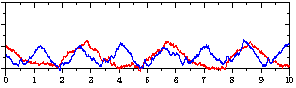
\includegraphics[scale=2.5]{OriginCourbePaquetsSuccessifs_2Bar}}
\path(5.05,1.6);

\draw (2.5,0) node[below=-2mm]{$t \left[\seconde{}\right]$};
\draw (-0.1,0.85) node[rotate=90]{$n(\zsonde,t) \left[ \ua \right]$};

%\node at (0.4,0.85){(c)};
\node at (1.5,1.0){$\zsonde=\cm{175}$};

\draw[blue](2.1,0.7)--+(0.5,0.3)node[above right]{avec 2 miroirs mobiles};
%%%%%%%%%%%%%%%%%%%%%%%%%%%%%%%%%%%%%%%%%%%%%%%%%%%%%%%%%%%%%
%%%%%%%%%%%%%%%%%%%%%%%%%%%%%%%%%%%%%%%%%%%%%%%%%%%%%%%%%%%%%	
\end{tikzpicture}
\end{document}